%DO NOT MESS AROUND WITH THE CODE ON THIS PAGE UNLESS YOU %REALLY KNOW WHAT YOU ARE DOING
\chapter{Project Objectives} \label{Project Objectives}
\section{Project Objectives} \label{Project Objective}
Based on the above Chapters and information, our objectives are as follows:
\begin{enumerate}[(a)]
  \item To design and implement a capture and detection system for manufactured and DIY drones from their frequency signatures using Software Defined Radios like PlutoSDR, NI-SDR etc.
  \item To design and implement a machine-learning algorithm to analyse the captured data and classify the signals as drone and non-drone signals.
  \item To use the output of the machine learning algorithm to find the frequency of operation of the drone and send out a jamming signal to hinder its operations.
\end{enumerate}

\section{Project Methodology} \label{Project Methodology}

\subsection{Data Creation and Preparation}

Data creation and preparation involve the capture of the signals and converting them into usable datasets which can be later used by the machine learning algorithm. This entails the following processes :
\begin{figure}[H]
  \centering
  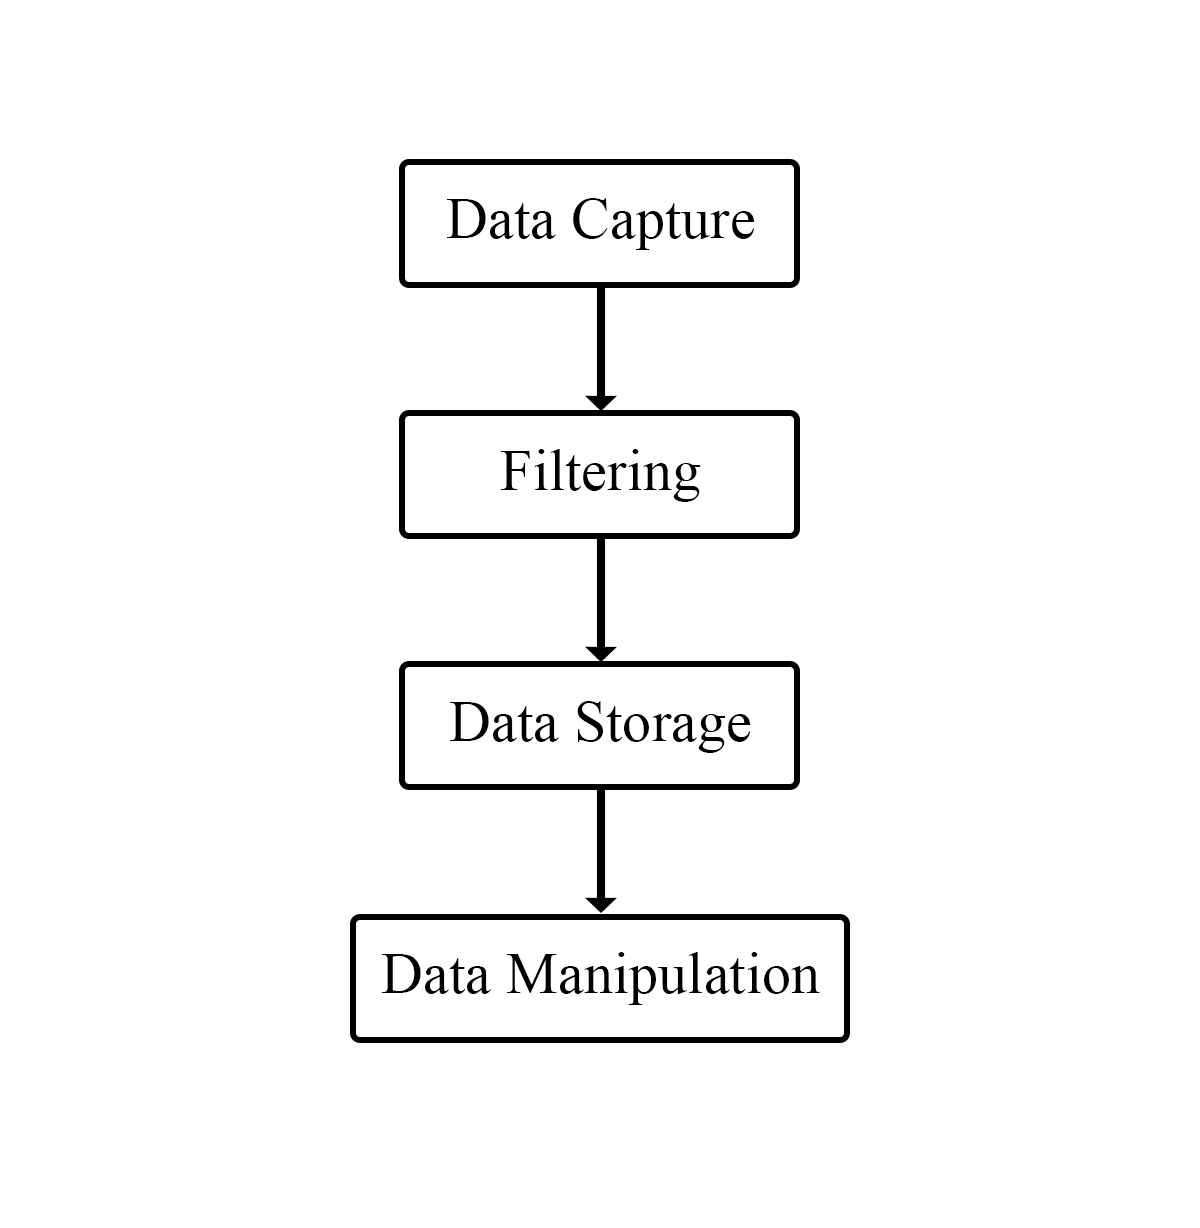
\includegraphics[width=0.5\textwidth]{dataCreationAndPreparation.png}
  \caption{Data creation pipeline}
\end{figure}


\begin{enumerate}
  \item \underline {Data Capture}
\begin{itemize}
    \item Data capture is the process of collecting data that will be processed and later used to fulfil certain purposes.
    \item In our case, we shall make use of a Software Defined Radio to Capture the frequency spectrum for further analysis. This process involves setting up the capture device on the platform used for storing the data. This is done by installing the required libraries and API’s, calibrating the receiver and detecting the signal intended to be captured.

    \item This requires intensive research about the frequencies that are used for drone communication. Finding an optimum range to be captured to avoid the capture of the unnecessary spectrum and unwanted signals is extremely necessary. This is done to reduce the size of the dataset thus saving processing time.
\end{itemize}

  \item \underline {Filtering}
\begin{itemize}
    \item Filtering is the process that, completely or partially, suppresses unwanted components or features from a signal. This means removing some frequencies to suppress the interfering signals and to reduce the Background/ambient noise. In our case, even filtering the natural resonance of the software-defined radio is required to get a clean and usable spectrum scan.
    \item This can be done by using multiple methods. We plan to use a thresholding function on the captured signals to get rid of the unwanted low power signals which are usually ambient noise and disturbances.
    \item This also helps to get rid of empty datasets which purely contain noise. Thus helping to create more concise and useful datasets. After filtering, the captured data is sent to the next process that is data storage.
\end{itemize}
  \item \underline {Data storage}
\begin{itemize}
    \item Data storage is the process of storing the captured and filtered data in the required format which in our case is in the form of CSV files (comma separated values) using the Pandas library for ease of access and storage.
    \item The stored data is then sent to the Next step in the process that is the data manipulation process.
\end{itemize}

  \item \underline {Data Manipulation}
\begin{itemize}
   \item Data manipulation refers to the process of adjusting data to make it organised and easier to read. This might involve adding, deleting, and modifying the database. This is one of the main stages to get the data prepared for use by the model.
    \item In our case, data manipulation is done to make it easier for the machine learning model to process the data and make it useful for model training and testing. This is done by combining multiple CSV files generated during the previous stages and manipulating the data within to reduce the size of the files and organise them as per the requirements of the model.
    \item Training labels are also assigned during this stage. In machine learning, labelling is the process of identifying raw data and adding one or more meaningful and informative labels. This is done to provide context so that a machine learning model can learn from it. In our case, labels are used to indicate the difference between a drone and non-drone signals such as Wi-Fi and Bluetooth signals.
    \item The datasets obtained from this process are then split into Training sets and Evaluation sets which are then used for the machine learning process.
\end{itemize}
    \end{enumerate}

    \subsection{Machine learning model and Training}

    Once the data is in usable shape and format, the next step would be to form a machine learning model and to train it using the data prepared earlier by applying a range of techniques and algorithms and check its operation and accuracy and get a feasible output.

    \begin{figure}[H]
      \centering
      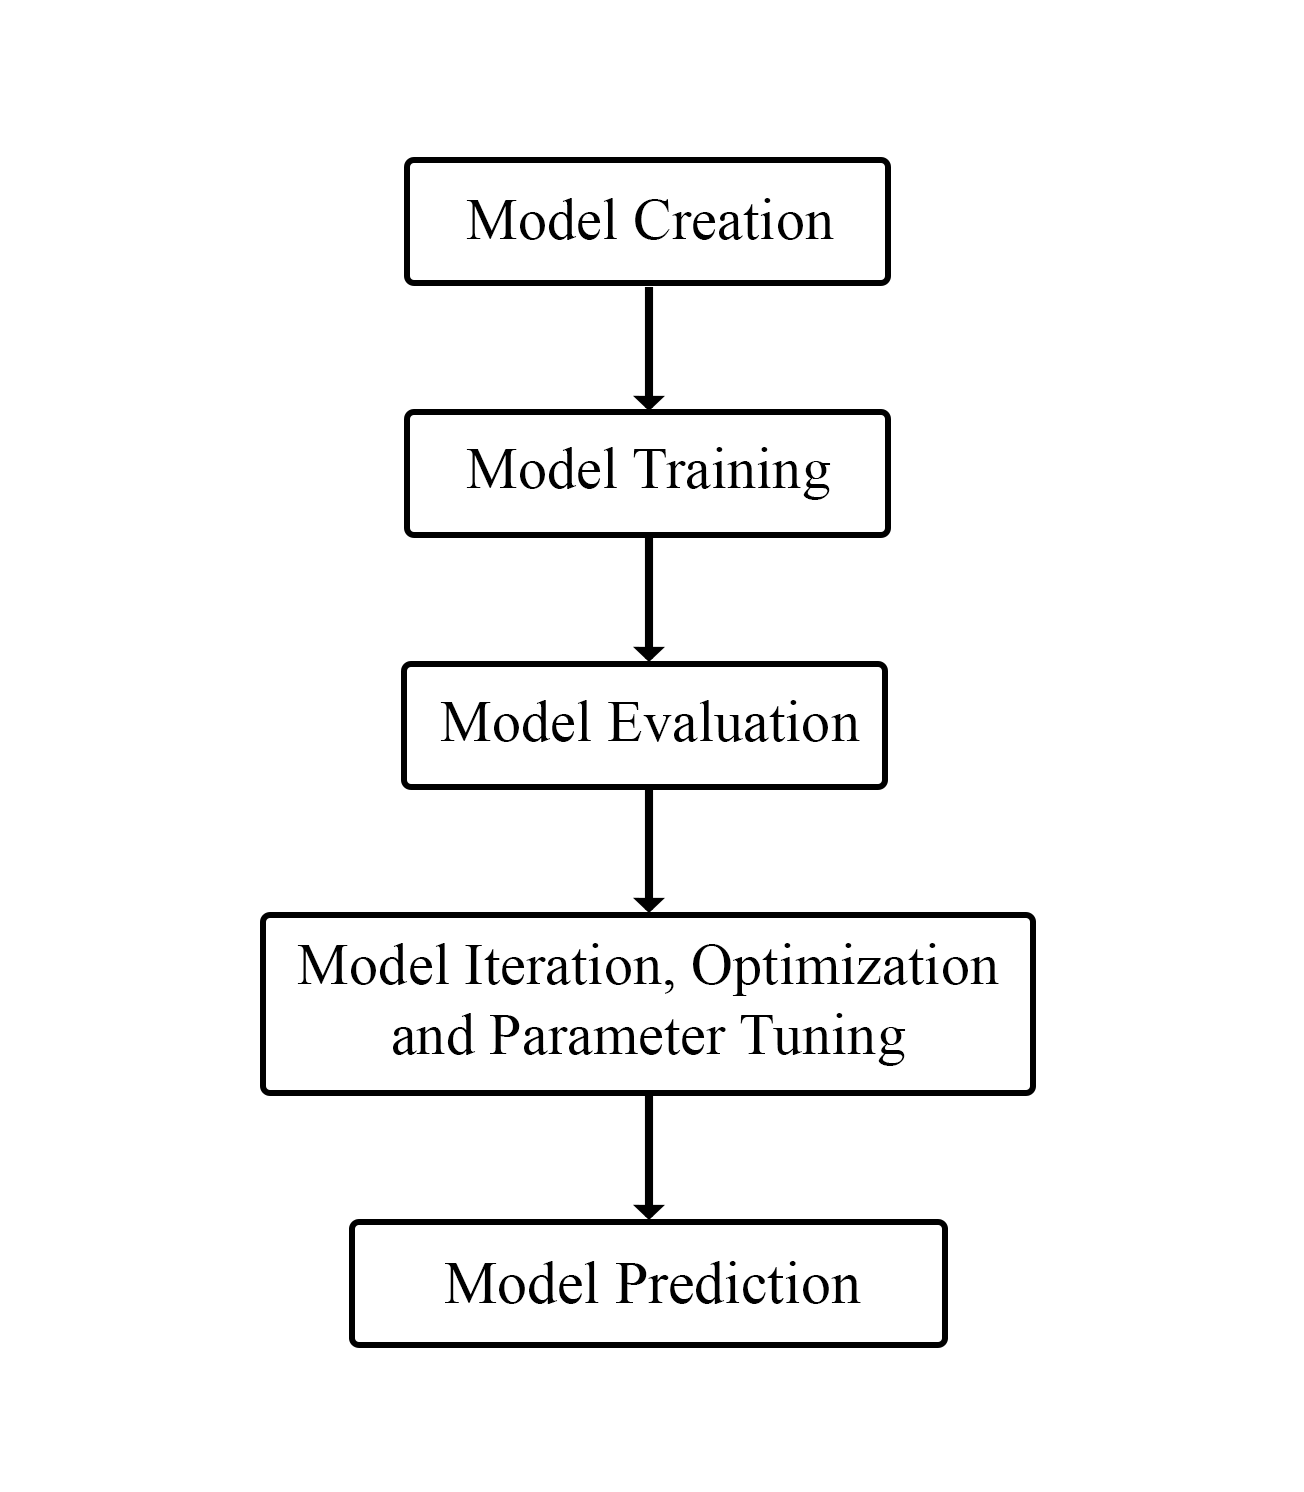
\includegraphics[width=0.5\textwidth]{MachineLearningModelAndTaining.png}
      \caption{Machine learning pipeline}
    \end{figure}

    This phase includes model technique selection and application, setting model parameters and adjustments, algorithm selection, Classification, model training, model evaluation, development and testing, model validation, and optimization of the model.
    \begin{enumerate}
      \item \underline {Model creation}
        \begin{itemize}
          \item Model creation includes selecting the right algorithm based on the objectives and the data available, Configuring , tuning the hyperparameters for optimal performance and determining a method of iteration. This is done to attain the best hyperparameters and identifying the features that could provide the best results.
          \item In our case, we will be using supervised learning to build the model which works on the basis of classification.
        \end{itemize}

      \item \underline {Model Training}
        \begin{itemize}
          \item Here the goal is to make sure that correct predictions are made as often as possible. Training a model simply means determining appropriate weights and the bias from labelled data using the training sets generated earlier.
          \item In supervised learning, a machine learning algorithm builds a model by examining many examples and attempting to find a model that minimizes loss. Loss is the penalty for a bad prediction. That is, the loss is a number indicating how bad the model's prediction was on a single example. If the model's prediction is perfect, the loss is zero, otherwise, the loss is greater. The goal of training a model is to find a set of weights and biases that have a low loss.
        \end{itemize}

      \item \underline {Model evaluation}
        \begin{itemize}
          \item Model evaluation includes the evaluation of the performance of a machine learning model, which is an integral step to the whole process. The model evaluation aims to estimate the general accuracy of the model of future or unseen data. This is done using validation or evaluation data sets which are used to train the model with the goal of finding and optimizing the best model to solve the problem at hand and further tune the hyperparameters for optimal performance.
          \item Model evaluation can be considered the quality assurance of machine learning. Adequately evaluating the models performance against metrics and requirements determining how the model will work in the real world.
        \end{itemize}

      \item \underline {Model iteration, optimization and parameter tuning}
        \begin{itemize}
          \item Based on the results of the evaluation process, adjustments are made to the various hyperparameters such as the number of training steps, learning rate, initialization of the weights
          \item This is done for multiple iterations or epochs so as to fine-tune the parameters and optimize the values of said parameters for improved performance and accuracy.
        \end{itemize}

      \item \underline {Prediction using the Model}
        \begin{itemize}
          \item Once the results of the model are satisfactory and the accuracy is acceptable, the model can be implemented in the real world for the sole purpose it was designed for and can start making predictions and get practicals outputs based on all the training, optimization and work put into the model.
        \end{itemize}
    \end{enumerate}
